\documentclass[11pt, letterpaper]{article}
\usepackage{graphicx}
\usepackage[export]{adjustbox}
\usepackage{hyperref}
\usepackage{xcolor}
\graphicspath{{images/}}
\usepackage[a4paper, total={6in, 8in}]{geometry}
\usepackage{tabularx}
\usepackage{float}


\title{\textbf {Audio classification with machine learning} \\ \large Introduction to Machine Learning 2024/2025Z}

\author{Łukasz Górski \\ Piotr Iśtok \\ Piotr Jacak \\ Stanisław Janowicz \\ Marcin Falkowski}

\date{Styczeń 2025}


\begin{document}
\maketitle

\newpage
\tableofcontents
\newpage

\section{Abstract}

The task we will be attempting to solve in this project is a binary recognition problem, meaning that the program's main function is to transform a given input into either 1 or 0, depending on certain properties and conditions. Specifically, the input will consist of a single audio file, either uploaded directly or recorded on a recorder with a microphone by the program. We will transform this audio file into a spectrogram and, after cleaning and pre-processing, pass it into the model to determine its membership in class one, representing the people who are granted access, or class zero, or the people who are denied.

The intended use of this project is on a voice-based intercom device that must discern whether a person has the authority to enter restricted areas.

\section{Introduction}

In this section we present some useful background information on audio classification and on the more technical aspects of the project.

\subsection{Audio Classification}
 Audio classification is a machine learning task that involves identifying and tagging audio signals into different classes or categories. In our case, this is done through the analysis of spectrograms of the files provided, since analysis of images is used much more frequently in the field of machine learning.

 Our data set is the \href{https://www.kaggle.com/datasets/psyreddy07/daps-data}{DAPS} set, consisting of .wav files of 20 speakers reading 5 scripts each, averaging at about 14 and a half minutes.

 Of those 20 speakers, F1, F7, F8, M3, M6, M8, are chosen as class 1, and the other speakers form class 0.

 \subsection{Convolutional Neural Networks}
 The model used is a Convolutional Neural Network (CNN), which is a common type of deep learning network employed in tasks of recognition, especially image processing. It consists of an input layer, a number of hidden layers, and an output layer. In our program, the output layer is binary, since we only have 2 classes.

 We chose the \verb|pytorch| library to implement our model.

\section{Cleaning and pre-processing}

\subsection{Preprocessing}
Effective preprocessing of audio data is a critical step in achieving high-quality features for machine learning models. In this project, preprocessing ensures uniformity across audio samples and eliminates irrelevant segments.
\subsubsection{Sample Rate}
In speech-related tasks, consistency in the sample rate is vital to ensure that all audio files have the same temporal resolution. We decided to set the base sample rate to 16kHz (Wideband frequency), because it is used in most modern VoIP (Voice over Internet Protocol) and is a extension over standard 8kHz narrowband. For us it was perfect balance between computational efficiency and retaining the critical sampling frequency.
\subsubsection{Removing Silent Parts}
Silence in audio fragments often contains no meaningful information for speaker recognition and can introduce noise or inflate the data size unnecessarily. To address this, silent parts of the audio were detected and removed during preprocessing. This step ensures that the input to the model focuses solely on speech, improving training efficiency and performance.

\subsection{Cleaning}
In machine learning applications that involve audio data, such as speaker identification, the quality of the input signal is critical. Background noise can obscure important voice features, which can lead to reduced model performance. One way of overcoming this issue and improving SNR (signal to noise ratio) is denoising data using spectral gating. It works by computing a spectrogram of a signal (and optionally a noise signal) and estimating a noise threshold (or gate) for each frequency band of that signal/noise.
That threshold is used to compute a mask, which gates noise below the frequency-varying threshold. The main reasons why it is a good option for reducing noise are:
\begin{itemize}
    \item \textbf{Preservation of signal features:}
        Spectral gating works in the frequency domain, selectively weakening noise-dominated frequencies, keeping the structure of our target signal (voice) mostly intact.
    \item \textbf{Flexibility:}
        The method uses a noise profile derived from a sample with only background noise, which allows our program to adapt to different environments such as street noise, electrical noise and reverberation. Because of it our code is simple without any noticeable performance drop.
    \item \textbf{Ease of use:}
        This method of denoising is implemented in the free-to-use Python library called "noisereduce", keeping our solution easily reproducible and can be seamlessly integrated into our pipeline.
\end{itemize}
Unfortunately, spectral gating also has its drawbacks. The biggest one is that, for it to work there needs to be a noise sample provided, which can be for us sometimes impossible to distinguish. That's why in that case our denoising step in pipeline will use band-stop filter, implemented with Butterworth filter. The main advantages of it are:
\begin{itemize}
    \item \textbf{No need for a noisy sample:}
        This filter always removes lower frequencies, so urban sounds can be easily eliminated, without the need of noisy sample.
    \item \textbf{Preservation of higher frequencies:}
        The Butterworth filter's characteristic smooth frequency response ensures minimal distortion in the preserved higher frequencies.
    \item \textbf{Preprocessing Simplicity:}
        This approach is computationally efficient and easy to implement.
\end{itemize}
The reason why it is not used all the time is that it has many limitations. It is not ideal for broadband noise. It may not effectively remove all of it. The other one is that it overlaps with voice frequencies, so it can also attenuate it resulting in reduced intelligibility.\\We also considered using deep learning for audio cleaning, as it has shown great potential by leveraging neural networks to learn complex mappings between noisy and clean audio signals. However, we came to the conclusion that it is too advanced a tool to remove such simple noises and two methods described before are efficient enough.

\subsection{Spectrograms}
In speaker recognition tasks, the selection of an appropriate feature extraction method is crucial. The acoustic properties of human speech vary widely and capturing these nuances effectively is essential for accurate classification. Among many methods for converting raw audio signals into a form suitable for machine learning, it was imposed on us to use spectrograms. We created three types, however in the final version only one of three listed down below methods is used.
\begin{itemize}
    \item \textbf{Regular Spectrogram}
        This method computes the spectrogram by applying the Short-Time Fourier Transform (Stft) to the audio signal. It visualizes how the signal's frequency content varies over time. While this approach provides an accurate representation of raw frequency components, it does not consider the perceptual differences in how humans interpret sound.
    \item \textbf{Spectrogram with adjustable parameters and dB scale}
        This method allowed us to changed parameters such as FTT size, window size and hop size. However tweaking those parameters didn't bring any improvements. The biggest advantage of this method compare to the previous one is dB scaling of spectrogram. Because of that more features were clearly shown.
    \item \textbf{Mel Spectrogram}
        The mel spectrogram method transforms the audio signal into a representation that closely matches the human ear's sensitivity to frequency. It maps the frequencies to the mel scale, which emphasizes lower frequencies (important for speech) while de-emphasizing higher, less perceptible frequencies. By focusing on perceptually relevant features, the mel spectrogram strikes a balance between simplicity, efficiency, and effectiveness. It directly produces features well-suited for downstream models without requiring extensive manual adjustments. To no surprise, this method we had the best results so it is being used in final version.
\end{itemize}
Additionally all spectrograms are stored in grayscale to take up as little space as possible without loosing important data for further usage.

\section{Methodology}

\section{Exploratory Data Analysis}

Exploratory Data Analysis (or EDA for short) is the process of gathering information from the given data set before using it for the purposes of informed decision making later on. Since our data are in the form of .wav files, we use the \verb | scipy.io.wavfile |Python library to load it in order to analyze it by looking directly at the array representing it. This was our first attempt at EDA, and although the code itself runs quick, it gives us very little useful information. Namely, we only have access to the numbers: the minimum and maximum values of the array, the means, sample rates and the lengths of the files in each class. This is hardly enough - the length of an audio doesn't, and shouldn't, affect how is it classified.

Therefore, we make use of Python libraries that are more suited to accomplishing our goals. After presenting the audio in the form of spectrograms, we extract helpful details into a .csv file, which becomes the input of the next stages of EDA. The details shown in the .csv vary greatly from the simple values of the previous step and are of much greater importance to us. Here are the features that we managed to extract in this way: Person, sex, script, audio type, is a test set, class, and contrast. Let us explain them one by one:
\begin{itemize}
    \item Person - the person speaking in the audio, as described in the Data section,
    \item Gender - the gender of the person (either male or female),
    \item Script - the script read in the audio,
    \item Audio Type - type of audio (either cleanraw, ipadflat, ipad, or iphone)
    \item Is Test Set - a binary value describing whether the file was used in training the model or testing it,
    \item Class - 0 or 1, as described in the Introduction
    \item Contrast - the contrast of the image.
\end{itemize}
Besides these values, there were five other features - average RGB values of the image as well as the Brightness and Saturation. However, as discussed in the Spectrograms section, the spectrograms were in grayscale, making all of these values equal to each other, and thus redundant. Because of this, we have decided to analyze only the mean redness value of the images with the understanding that it also signifies the other features from this section.

With this data, we can begin presenting the previously-numerical information visually, which makes the insights much more obvious to a human observer. We make use of the \verb|seaborn| library to generate histograms like the following:

\begin{figure}[H]
    \centering
    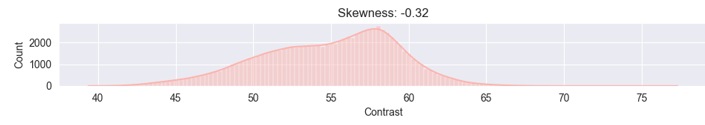
\includegraphics[width=1\linewidth]{image.png}
    \caption{Contrast distribution}
    \label{fig:enter-label}
\end{figure}

We can than utilize the same library to plot pairwise relationships in the data set, checking to what degree two variables are correlated with each other. Using the \verb|heatmap| function, we get the following result:

\begin{figure}[H]
    \centering
    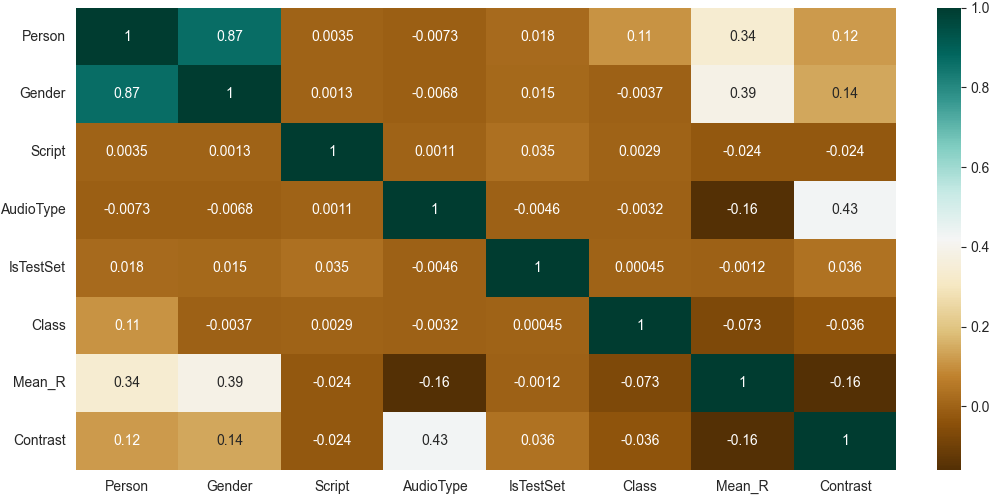
\includegraphics[width=1\linewidth]{pairplot.png}
    \caption{Pairwise relationships in the data set}
    \label{fig:enter-label}
\end{figure}

Lower values indicate a negative correlation between two variables, while values closer to 1 mean a positive association. From this heatmap, we can conclude that the Gender and Person variables are correlated, which means that the data set isn't split evenly between male and female recordings. This is a valuable insight, since it might affect model - if we chose the training set from the original data at random, the model might be worse at classifying one gender than the other.

Fortunately, looking at the value of the intersection between Gender and IsTestSet (0.015), the test set itself is fairly balanced.

\section{Cleaning and pre-processing}
\section{Models used}
\section{Results}

\end{document}